\chapter{Appendix }




\begin{table}[]
\caption{Current-based LIF neuron parameters used for the converted CNN}
\centering
\label{cnnlifparam}
\begin{tabular}{|ll|}
\hline
Resting potential    		& -65 mV 		    \\
Membrane Capacity    		& 1.0 nF 		     \\
Membrane time constant    	& 20.0 ms		             \\
Refractory period     		& 1.0 ms		                 \\
Offset current    			& 0.0 nA		              \\
Reset potential     		& -65.0 mV 	               \\
Spike threshold     		& -50.0 mV          \\\hline
\end{tabular}
\end{table}

\begin{table}[]
\caption{Current-based LIF neuron parameters used for the converted DBN}
\centering
\label{cubalifparam}
\begin{tabular}{|ll|}
\hline
Resting potential    		& -65 mV 		    \\
Membrane Capacity    		& 1.0 nF 		     \\
Membrane time constant    	& 1.0 ms		             \\
Refractory period     		& 10.0 ms		                 \\
Offset current    			& 1.0 nA		              \\
Reset potential     		& -53.0 mV 	               \\
Spike threshold     		& -52.0 mV          \\\hline
\end{tabular}
\end{table}


\begin{table}[]
\caption{Conductance-based LIF neuron parameters used for the converted DBN}
\centering
\label{cobalifparam}
\begin{tabular}{|ll|}
\hline
Resting potential    			& -65 mV 		    \\
Membrane Capacity    			& 1.0 nF 		     \\
Membrane time constant    		& 20.0 ms		             \\
Refractory period     			& 10.0 ms		                 \\
Offset current    				& 1.0 nA		              \\
Reset potential     			& -53.0 mV 	               \\
Spike threshold     			& -52.0 mV          \\
Inhibitory reversal potential  & 90.0 mV	              \\
Excitatory reversal potential  & -0.0 mV 	               \\\hline
\end{tabular}
\end{table}
   
 \begin{figure}[h!]
	\centering
	\begin{subfigure}[t]{.55\textwidth}
  		\centering
  		\includegraphics[width=.9\linewidth]{imgs/app/inhib_no.png}
  		\caption{Spike without lateral inhibition.}
  		\label{fig:sub1}
	\end{subfigure}%
	
	\begin{subfigure}[t]{.55\textwidth}
  		\centering
  		\includegraphics[width=.9\linewidth]{imgs/app/inhib_small.png}
  		\caption{Spike with small lateral inhibition.}
  		\label{fig:sub2}
	\end{subfigure}
	
	\begin{subfigure}[t]{.55\textwidth}
  		\centering
  		\includegraphics[width=.9\linewidth]{imgs/app/inhib_big.png}
  		\caption{Spike with big lateral inhibition.}
  		\label{fig:sub2}
	\end{subfigure}
	\caption{Spikes in a hidden layer of a spiking RBM with lateral inhibition. As the lateral inhibition increases, the activity becomes more sparse. In the case with big inhibitory weights, there are a few neurons dominating the activity allowing only a few different states of the network and thus poor mode switching in a training step. In a network with small inhibitory weights, there is sparse activity, but the the network visits many different states in a simulation step and shows sufficient mode mixing. }
	\label{fig:dbnmixing}
\end{figure}
   
 \begin{figure}[h!]
	\centering
	\begin{subfigure}[t]{.49\textwidth}
  		\centering
  		\includegraphics[width=.4\linewidth]{imgs/spike_dbn.png}
  		\label{fig:sub1}
  		\caption{DBN with distinct RBM layers.}
	\end{subfigure}%
	\begin{subfigure}[t]{.49\textwidth}
  		\centering
  		\includegraphics[width=.9\linewidth]{imgs/app/DBN_sp.png}
  		\label{fig:sub1}
	\end{subfigure}%
	
	
	\begin{subfigure}[t]{.49\textwidth}
  		\centering
  		\includegraphics[width=.4\linewidth]{imgs/spike_dbm.png}
  		\label{fig:sub1}
  		\caption{DBN with distinct RBM layers, with bidirectional weights.}
	\end{subfigure}%
	\begin{subfigure}[t]{.49\textwidth}
  		\centering
  		\includegraphics[width=.9\linewidth]{imgs/app/DBM_sp.png}
  		\label{fig:sub2}
	\end{subfigure}
	
	
	\begin{subfigure}[t]{.49\textwidth}
  		\centering
  		\includegraphics[width=.50\linewidth]{imgs/app/dbn_np_arch.png}
  		\label{fig:sub1}
  		 \caption{DBN with RBM directly stacked to each other.}
	\end{subfigure}%
	\begin{subfigure}[t]{.49\textwidth}
  		\centering
  		\includegraphics[width=.9\linewidth]{imgs/app/DBN_np_sp.png}
  		\label{fig:sub2}
	\end{subfigure}
	\caption{Activity in the visible layer of the top RBM in a DBNs with different architectures. The first two architectures model separate RBM layers which are stacked by one-on-one forward connections from the hidden layer of the bottom RBM to the visible layer of the top RBM, while in the last architecture, the RBMs are directly stacked, i.e. the hidden layer of the bottom RBM is the visible layer of the top RBM. While in the top two architectures, there are hardly any differences and the input is modelled correctly, due to top down influences the output of the bottom RBM gets distorted by activity in the hidden layer of the top RBM.}
	\label{fig:spikingdbnarch}
\end{figure}


 \begin{figure}[h!]
	\centering
	\begin{subfigure}[t]{.24\textwidth}
  		\centering
  		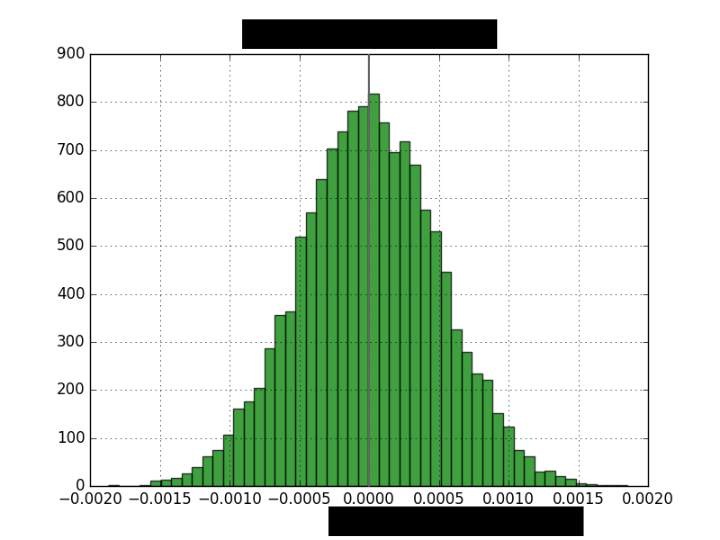
\includegraphics[width=.9\linewidth]{imgs/app/nest/w_hist_conv1.png}
  		\caption{Weights at the beginning.}
  		\label{fig:sub1}
	\end{subfigure}%
	\begin{subfigure}[t]{.24\textwidth}
  		\centering
  		\includegraphics[width=.9\linewidth]{imgs/app/nest/w_hist_conv2.png}
  		\caption{Weights after first positive phase.}
  		\label{fig:sub2}
	\end{subfigure}
	\begin{subfigure}[t]{.24\textwidth}
  		\centering
  		\includegraphics[width=.9\linewidth]{imgs/app/nest/w_hist_conv3.png}
  		\caption{Weights after first negative phase.}
  		\label{fig:sub2}
	\end{subfigure}
	\begin{subfigure}[t]{.24\textwidth}
  		\centering
  		\includegraphics[width=.9\linewidth]{imgs/app/nest/w_hist_conv4.png}
  		\caption{Weights after a few training steps.}
  		\label{fig:sub2}
	\end{subfigure}
	

	\begin{subfigure}[t]{.24\textwidth}
  		\centering
  		\includegraphics[width=.9\linewidth]{imgs/app/nest/spikes_conv.png}
  		\caption{Spikes activity development.}
  		\label{fig:sub2}
	\end{subfigure}
	
	
	\begin{subfigure}[t]{.24\textwidth}
  		\centering
  		\includegraphics[width=.9\linewidth]{imgs/app/nest/w_hist_conv_lr.png}
  		\caption{Weights after training with different positive and negative learning rates.}
  		\label{fig:sub2}
	\end{subfigure}
	
	\begin{subfigure}[t]{.24\textwidth}
  		\centering
  		\includegraphics[width=.9\linewidth]{imgs/app/nest/w_hist_normal.png}
  		\caption{Weights without any synchronization.}
  		\label{fig:sub2}
	\end{subfigure}	
	
	\caption{Weights development for eCD with synchronous weight updates. The first column shows the development. After the positive the weights increased a lot, which leads to a high decrement during the negative which leads to a "dying out" of the spikes, which is visualized in the second column. Using an increased positive phase with a higher learning rate, does not solve the problem and leads to a division of the weights into a few very positive weights and many negative weights. In contrast to this a "normal" weight distribution without any weight synchronization in presented in the last column. }
	\label{fig:ecdnest}
\end{figure}

